\section{Task-Aware Robustness and Sensitivity Visualization}\label{sec:robust}
Figure~\ref{fig:labelpolicy} makes target-definition dependence explicit. Each interval is a bootstrap confidence interval \emph{for a different analysis population}, not a paired estimator comparison on identical cases. The original score and direction are held fixed. The primary duplicate-rate interval includes chance ranking; the broader runner intervals do not. This indicates label-selection sensitivity, not validated semantic-defect classification.

\begin{figure}[t]
\centering
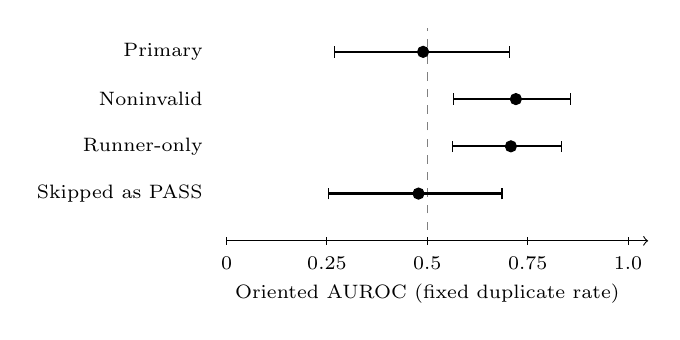
\begin{tikzpicture}[x=5.1cm,y=0.60cm, font=\scriptsize]
\draw[->] (0,0)--(1.05,0);
\foreach \x in {0,0.25,0.5,0.75,1.0} {
  \draw (\x,-0.08)--(\x,0.08);
  \node[anchor=north] at (\x,-0.13) {\x};
}
\draw[dashed,gray] (0.5,0.23)--(0.5,4.5);
\node[anchor=east] at (-0.035,4) {Primary};
\node[anchor=east] at (-0.035,3) {Noninvalid};
\node[anchor=east] at (-0.035,2) {Runner-only};
\node[anchor=east] at (-0.035,1) {Skipped as PASS};
\foreach \lo/\hi/\point/\y in {
  0.269582/0.705747/0.489470/4,
  0.565309/0.856875/0.720528/3,
  0.562218/0.834433/0.708096/2,
  0.254538/0.685949/0.478052/1
}{
  \draw[thick] (\lo,\y)--(\hi,\y);
  \draw (\lo,\y-0.12)--(\lo,\y+0.12);
  \draw (\hi,\y-0.12)--(\hi,\y+0.12);
  \filldraw (\point,\y) circle (2pt);
}
\node[anchor=north] at (0.5,-0.70) {Oriented AUROC (fixed duplicate rate)};
\end{tikzpicture}
\caption{Duplicate-terminal-rate AUROC (point) and task-cluster bootstrap 95\% confidence interval (whiskers) under four frozen but different label policies. Dashed line denotes 0.5. Inputs: corrected Step 10 v2.}
\label{fig:labelpolicy}
\end{figure}

Step 11 robustness checks were computed \emph{after} the main AUROCs had been seen. They are therefore exploratory interpretation stress tests, not confirmatory improvements to the frozen methodology. Table~\ref{tab:robustness} shows how weighting and restricting comparable units changes the duplicate rate's score.

\begin{table}[t]
\caption{Exploratory duplicate-rate robustness under distinct analysis units; not held-out prediction.}
\label{tab:robustness}
\centering
\resizebox{\columnwidth}{!}{%
\begin{tabular}{lcc}
\toprule
Descriptive analysis & Primary & Runner-only\\
\midrule
Run-level AUROC &0.489&0.708\\
Task-macro AUROC$^\dagger$ &0.522&0.741\\
Within-project AUROC$^\ddagger$ &0.390&0.738\\
Leave-one-positive-task-out range &0.382--0.620&0.683--0.759\\
Positive task IDs &5&15\\
\bottomrule
\end{tabular}}
\vspace{1mm}

{\footnotesize $^\dagger$Unanimously labeled tasks only; discordant tasks excluded. $^\ddagger$Pairs from different tasks in the same project. Neither method measures accuracy on previously unseen tasks.}
\end{table}

For the primary target, task-macro AUROC is 0.522, within-project AUROC is 0.390, and removing each positive task family gives run-level estimates from 0.382 to 0.620. Which task appears in the primary positive set therefore matters greatly. For the runner-only sensitivity, the corresponding leave-one-positive-task-out range is 0.683 to 0.759 across 15 distinct positive tasks; this does not prove those broader positives are true semantic defects.

An explicitly post-hoc trajectory-length comparator also yielded AUROC 0.660 under the primary policy, while duplicate rate versus step count had Spearman correlation $-0.112$. These descriptive checks were not selected or calibrated before outcomes and therefore cannot be interpreted as a new validated predictor. Task-difficulty confounding has not been eliminated. All exploratory inputs are versioned in the public Step 11 robustness JSON.
